\documentclass[12pt,letterpaper]{article}
\usepackage[utf8]{inputenc}
\usepackage[version=3]{mhchem}
\usepackage[journal=jacs]{chemstyle}
\usepackage{amsmath}
\usepackage{amsfonts}
\usepackage{amssymb}
\usepackage{makeidx}
\usepackage{xcolor}
\usepackage[stable]{footmisc}
\usepackage[section]{placeins}
\usepackage{longtable}
\usepackage{array}
\usepackage{xtab}
\usepackage{multirow}
\usepackage{colortab}
\usepackage{siunitx}
\usepackage{graphicx}
\usepackage{caption} % for \captionof

\sisetup{mode=text, output-decimal-marker = {,}, per-mode = symbol, qualifier-mode = phrase, qualifier-phrase = { de }, list-units = brackets, range-units = brackets, range-phrase = --}
\DeclareSIUnit[number-unit-product = \;] \atmosphere{atm}
\DeclareSIUnit[number-unit-product = \;] \pound{lb}
\DeclareSIUnit[number-unit-product = \;] \inch{"}
\DeclareSIUnit[number-unit-product = \;] \foot{ft}
\DeclareSIUnit[number-unit-product = \;] \yard{yd}
\DeclareSIUnit[number-unit-product = \;] \mile{mi}
\DeclareSIUnit[number-unit-product = \;] \pint{pt}
\DeclareSIUnit[number-unit-product = \;] \quart{qt}
\DeclareSIUnit[number-unit-product = \;] \flounce{fl-oz}
\DeclareSIUnit[number-unit-product = \;] \ounce{oz}
\DeclareSIUnit[number-unit-product = \;] \degreeFahrenheit{\SIUnitSymbolDegree F}
\DeclareSIUnit[number-unit-product = \;] \degreeRankine{\SIUnitSymbolDegree R}
\DeclareSIUnit[number-unit-product = \;] \usgallon{galón}
\DeclareSIUnit[number-unit-product = \;] \uma{uma}
\DeclareSIUnit[number-unit-product = \;] \ppm{ppm}
\DeclareSIUnit[number-unit-product = \;] \eqg{eq-g}
\DeclareSIUnit[number-unit-product = \;] \normal{\eqg\per\liter\of{solución}}
\DeclareSIUnit[number-unit-product = \;] \molal{\mole\per\kilo\gram\of{solvente}}
\usepackage{cancel}
\usepackage{graphicx}
\usepackage{lmodern}
\usepackage{fancyhdr}
\usepackage[left=4cm,right=2cm,top=3cm,bottom=3cm]{geometry}

\usepackage[backend=bibtex,style=chem-acs,biblabel=dot]{biblatex}
\addbibresource{references.bib}

\usepackage{titlesec}
\usepackage{enumitem}
\titleformat*{\section}{\bfseries\large}
\titleformat*{\subsection}{\bfseries\normalsize}

\usepackage{float}
\floatstyle{plaintop}
\newfloat{anexo}{thp}{anx}
\floatname{anexo}{Anexo}
\restylefloat{anexo}
\restylefloat{figure}

\usepackage[margin=10pt,labelfont=bf]{caption}

\usepackage{todonotes}

\usepackage[colorlinks=true, 
            linkcolor = blue,
            urlcolor  = blue,
            citecolor = black,
            anchorcolor = blue]{hyperref}


\begin{document}
\renewcommand{\labelitemi}{$\checkmark$}

\renewcommand{\CancelColor}{\color{red}}

\newcolumntype{L}[1]{>{\raggedright\let\newline\\\arraybackslash}m{#1}}

\newcolumntype{C}[1]{>{\centering\let\newline\\\arraybackslash}m{#1}}

\newcolumntype{R}[1]{>{\raggedleft\let\newline\\\arraybackslash}m{#1}}

\begin{center}
	\textbf{\LARGE{Parallelization of 3D printer algorithm using Open-CL framework }}\\
	\vspace{7mm}
	\textbf{\large{Sharankumar Narayan Huggi (vipersnh)}}\\
	\vspace{4mm}
	\textbf{\large{University of Michigan}}\\
	\textbf{\large{EECS 587: Parallel Computing}}\\
	\textbf{\large{Professor: Quentin F. Stout}}\\
	\today
\end{center}

\vspace{7mm}

\section*{\centering Abstract}
3D printers are a pretty common name now-a-days among many engineers and do-it-yourself (DIY) enthusiasts. They come in variety of packages and formats, and print from different plastic materials. There are printers which can even print metal 3D objects. A major problem among the commercially available 3D printers, as well as DIY printers is that they take very long time to print 3D objects. This time not only depends on how much plastic material is infused into the 3D object but also on the complexity of the 3D object. Professor Chinedum Okwudire from the Mechanical Engineering Department at University of Michigan has designed a complex algorithm to reduce the time taken by 3D printers for printing 3D objects up-to 50 percent. However, running the algorithm to generate the sequence for 3D printer itself takes quite a lot of time. In this paper I address the implementation of the complex algorithm using parallel computing and Open-CL frameworks to reduce the algorithm execution time.

\section{Introduction}
Today we live in a world where technology drives our day-to-day activities and our surroundings. 3D printers are a set of technologies which are making big impact on our everyday lives. 3D printers help in rapid prototyping of 3D objects which help designers of products have a first hand experience of their products even before their actual production. They help students take their Computer Aided Design (CAD) models to reality without much effort which was not possible before the invention of 3D printers.

Now that 3D printers have come into existence, human quest for making them faster, more accurate and durable takes them further than what they were designed to be. This process starts by identifying the performance parameters which can be optimized or made faster. One such parameter is time taken for printing a 3D object using a DIY 3D printer. 

A 3D printer mainly consists of motors which drive a print head in 3-dimensional space. The print head is composed of heating chamber which melts plastic material to be drawn in lines to produce a 3D print layer by layer. Another special motor draws the plastic material (which exists in the form of a thread) into the heating chamber to melt newer plastic and flush out molten plastic. The image in \ref{fig:representational_3d_printer} shows a representational 3D printer which can be used to correlate the concepts presented in the paper.

Most of the time consumed in a 3D printer comes from the speed at which the motors run & the speed at which the heating chamber melts plastic. The motors have a physical limit on their speed since they must be controlled at each step. Going beyond their speed limits in software results in them missing software step commands which results in deformed prints. Thus the available 3D printers are shipped with the software under utilizing the speed of motors to be safe from deformed prints. Prof. Okwudire algorithm combines advanced processing into 3D printer software which promises to increase the top speed at which 3D printers operate by pre-calculating jerks produced at top speed and optimizing that part in 3D printer software.

\begin{center}
   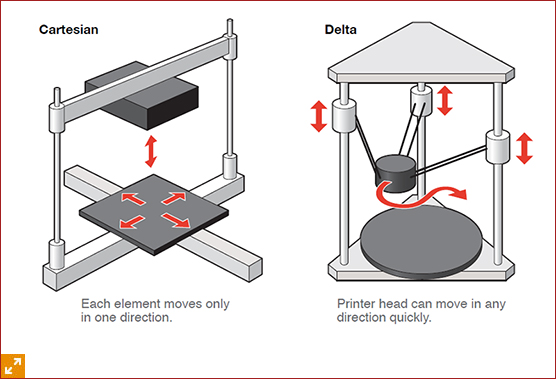
\includegraphics[scale=0.8]{images/cartesian-vs-delta.jpg}
   \captionof{figure}{Representational 3D Printer}
   \label{fig:representational_3d_printer}
\end{center}

\section{Motivation}
During the research phase of the professor, the algorithm for optimizing the speed of 3D printing was designed initially in MatLab & Simulink software provided by MathWorks Inc. Because MatLab & Simulink are very high level languages they are pretty CPU intensive for the work. Since it is a very inefficient task to run an algorithm in MatLab during production deployment once prototyping in MatLab works as expected, I took up this project to convert the implementation from MatLab to C++ and apply parallel computing algorithms for the processing part to improve the performance. Since I worked in the 3D project team's embedded systems implementation part, I'm very well aware of the concepts used in the whole project. This also forms a great optimization project to understand and implement parallelization concepts since computation time can be optimized using GPU processing.

\section{Related Work}
Since this project is a first of the kind, there is no previous work related to GPU optimization for 3D printer algorithm. A member from the Prof. Okwudire team tried to use multiprocessing library from Python to improve the performance of the algorithm, but it still falls short of the required speed ups which can be obtained using a GPU.

\section{Serial Architecture and Implementation}
The basic architecture of the project involves taking a 3D printer Gcode file and producing a binary output file which is used to drive the stepper motors. A Gcode file is a text file which contains the sequence of positions and directions for the different axes of the 3D printer where it needs to fill the molten plastic material to construct the 3D object. In a conventional 3D printer, the Gcode file is processed by a small embedded micro-controller which decides the commands to be sent to each of the axis motors step by step. The micro-controller generates a step and direction command for each stepper motor in the 3D printer.

For the implementation of faster 3D prints, Prof. Okwudire's algorithm sits between the Gcode file and the stepper command generation part to process the Gcode to generate the stepper commands. The architecture image as shown in \ref{fig:serial_algorithm} gives an overview of the process that is involved in the generation of the final ".bin" file. 

\begin{center}
   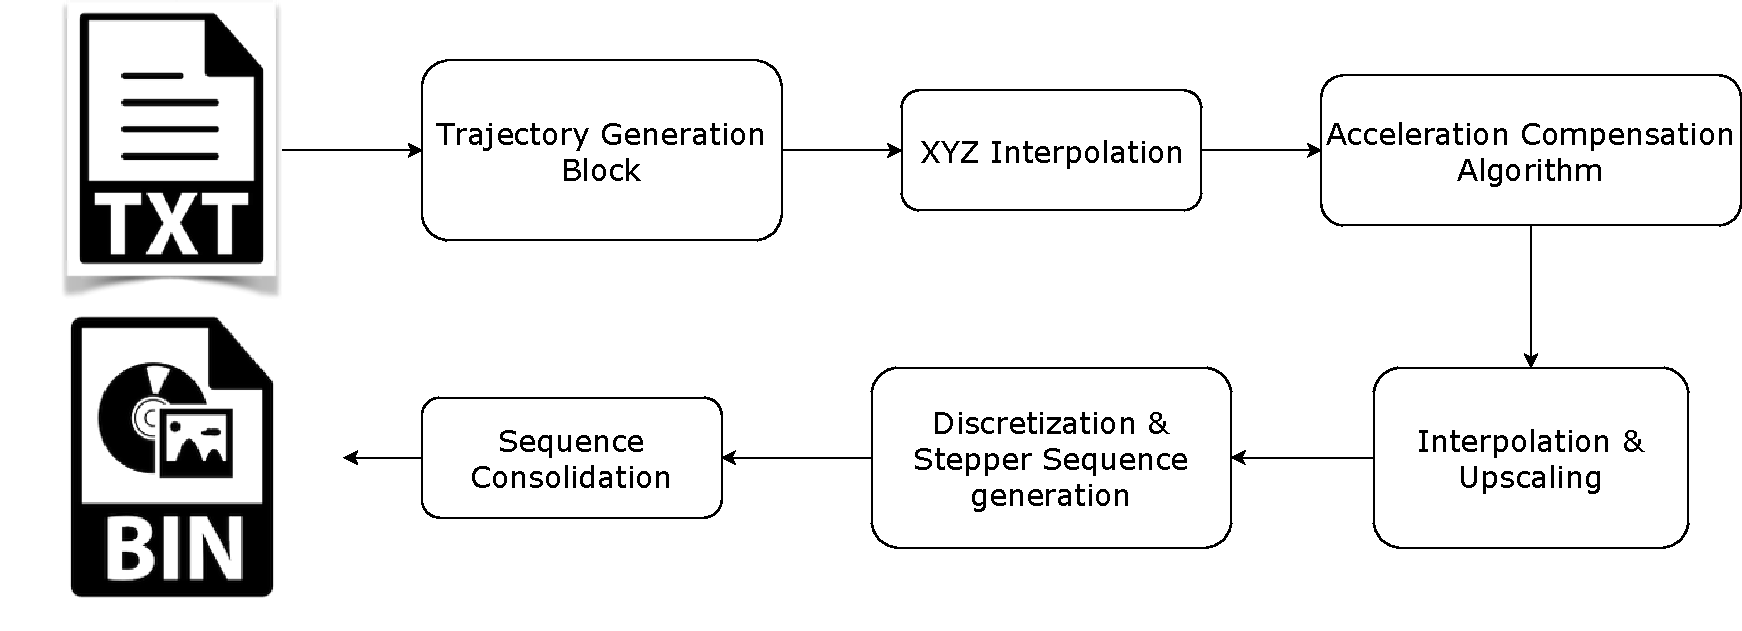
\includegraphics[scale=0.45]{images/serial-program.pdf}
   \captionof{figure}{Serial Algorithm Implementation}
   \label{fig:serial_algorithm}
\end{center}

\section{Validation and Verification}
For the purpose of verification of the serial implementation, I used the Python implementation provided by the researcher who works for Prof. Okwudire. By comparing the resulting output.bin files generated for five different Gcode 3D print files, I validated the serial program algorithm. This took most of the time during implementation since the design of C++ implementation was drastically different from the Python implementation.

\section{Parallel Architecture and Implementation}

\begin{center}
   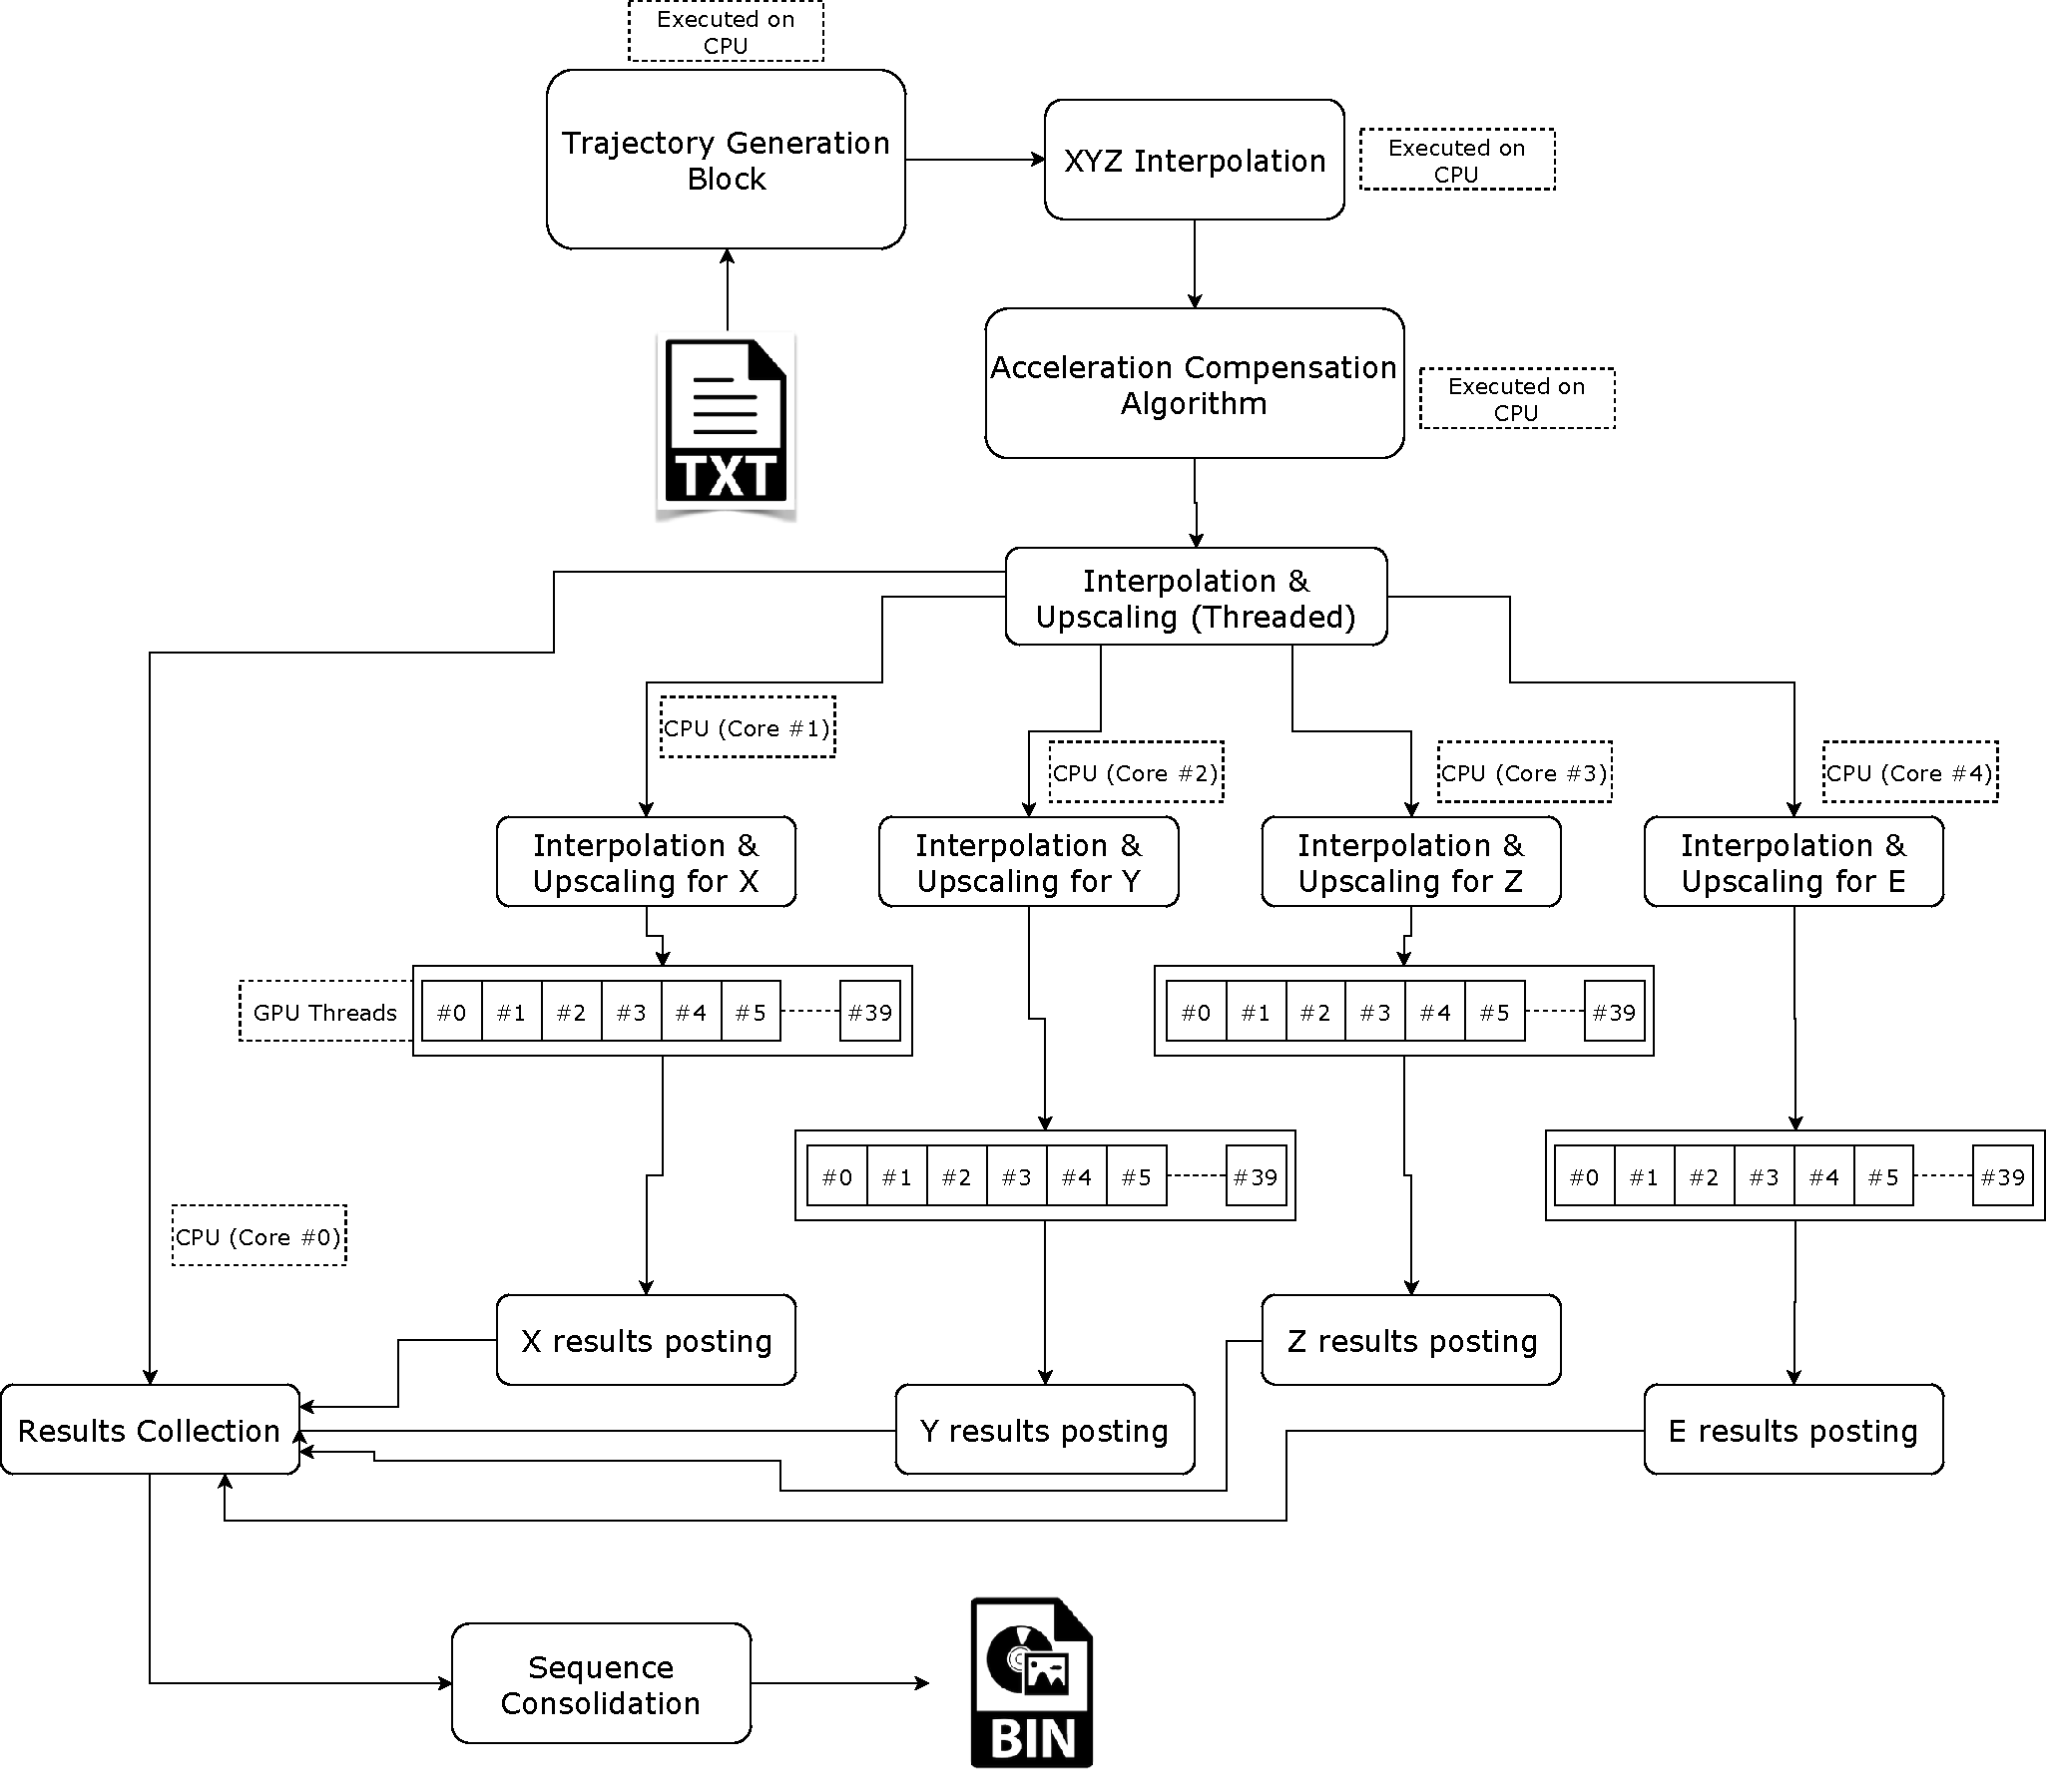
\includegraphics[scale=0.40]{images/parallel-program.pdf}
   \captionof{figure}{Paralleled Algorithm Implementation}
   \label{fig:parallel_algorithm}
\end{center}

\section{Performance Results}

\section{Conclusion}
The optimized implementations presented in this paper definitely prove to be useful in the 3D printing and DIY community. As can be seen from the results, the performance of the said algorithm increased by many folds by converting it from a Python based implementation to a C++ based implementation. This performance was further improved by adding in Open-CL framework. The implementation provided in this paper proves as a proof of concept for optimization of 3D printer related software algorithms to utilize GPU for faster processing. It also explores the repeated execution of certain instructions which makes it easier for parallelization of Gcode to stepper motor commands.
It also gives a highlight and in-depth code implementation for someone who wants to leverage Open-CL framework for faster processing using GPU architecture.

\section{Future Work}
The current implementation is focused on generating the final binary output file in a direct manner from the input Gcode file. However, according to the future implementation and usage of this algorithm according to Prof. Okwudire, we need to break the algorithm such that it generates the output sequence of stepper motor commands in an on-demand basis so as to efficiently use the storage space of the computing device involved, and providing best efficiency of the available computing power at hand.

\section{References\label{sec:references}}

\printbibliography[heading=none]

\end{document}
